\cardfrontfoot{Kapitel 20}

\begin{flashcard}[Struktur]{Nævn alle plankvadratiske komplekser}
\ce{[PtCl4]^{2-}}, \ce{[Ni(CN)4]^{2-}}, \ce{[Pt(NH3)2Cl2]}, \ce{[Ni(DMG)2]}, \ce{[Cu(NH3)4]^{2+}} samt øvrige platin og palladium komplekser.\\\vspace*{0.5cm}
Alle andre komplekser med fire ligander er tetraedriske.
\end{flashcard}

\begin{flashcard}[Struktur]{Opskriv for hver af $3d$ overgangsmetallerne de oxidationstrin hvor det danner forbindelser med oxygen}
\begin{tabular}{l*{8}{c}r}
Ox.			& Ti & V & Cr & Mn & Fe & Co & Ni & Cu \\
\hline
1			&  &  &  &  &  &  &  & X \\
2			& X & X &  & X & X & X & X & X \\
2 \& 3		&  &  &  & X & X & X &  & \\
3			& X & X & X & X & X &  &  & \\
4			& X & X & X & X &  &  & X & \\
5			&  & X &  &  &  &  &  & \\
6			&  &  & X &  &  &  &  & \\
7			&  &  &  & X &  &  &  & \\
\end{tabular}
\end{flashcard}

\begin{flashcard}[Egenskab]{Hvilke tre overgangsmetaller danne alle stabile oxyanioner i sur opløsning?}
\ce{VO4^{3-}}, \ce{CrO4^{2-}} og \ce{MnO4^{-}} triaden
\end{flashcard}

\begin{flashcard}[Egenskab]{Hvilke tre overgangsmetaller danner alle tetrachloro komplekser?}
Fe, Co og Ni triaden
\end{flashcard}

\begin{flashcard}[Fremstilling]{Opskriv reaktionsligninger for hvordan rent titanium og titaniumdioxid fremstilles industrielt}
\ce{TiO2 + 2C + 2Cl2 ->[\text{$\Delta$}] TiCl4 + 2CO}\\\vspace*{0.5cm}
\ce{TiCl4 + 2Mg ->[\text{$\Delta$}] Ti + 2MgCl2}\\
eller\\
\ce{TiCl4 + O2 ->[\text{$\Delta$}] TiO2 + 2Cl2}
\end{flashcard}

\begin{flashcard}[Egenskab]{Angiv den primære mineralkilde til chrom}
Chromit, \ce{FeCr2O4}
\end{flashcard}

\begin{flashcard}[Egenskab]{Forklar hvorfor chromat- og dichromationen ikke er farveløse}
Charge transfer til oxygen.
\end{flashcard}

\begin{flashcard}[Reaktion]{Angiv ammoniumdichromats spontane reaktion ved antændelse}
\ce{(NH4)2Cr2O7 -> Cr2O3 + N2 + 4H2O(g)}
\end{flashcard}

\begin{flashcard}[Struktur]{Tegn strukturen af dichromationen}
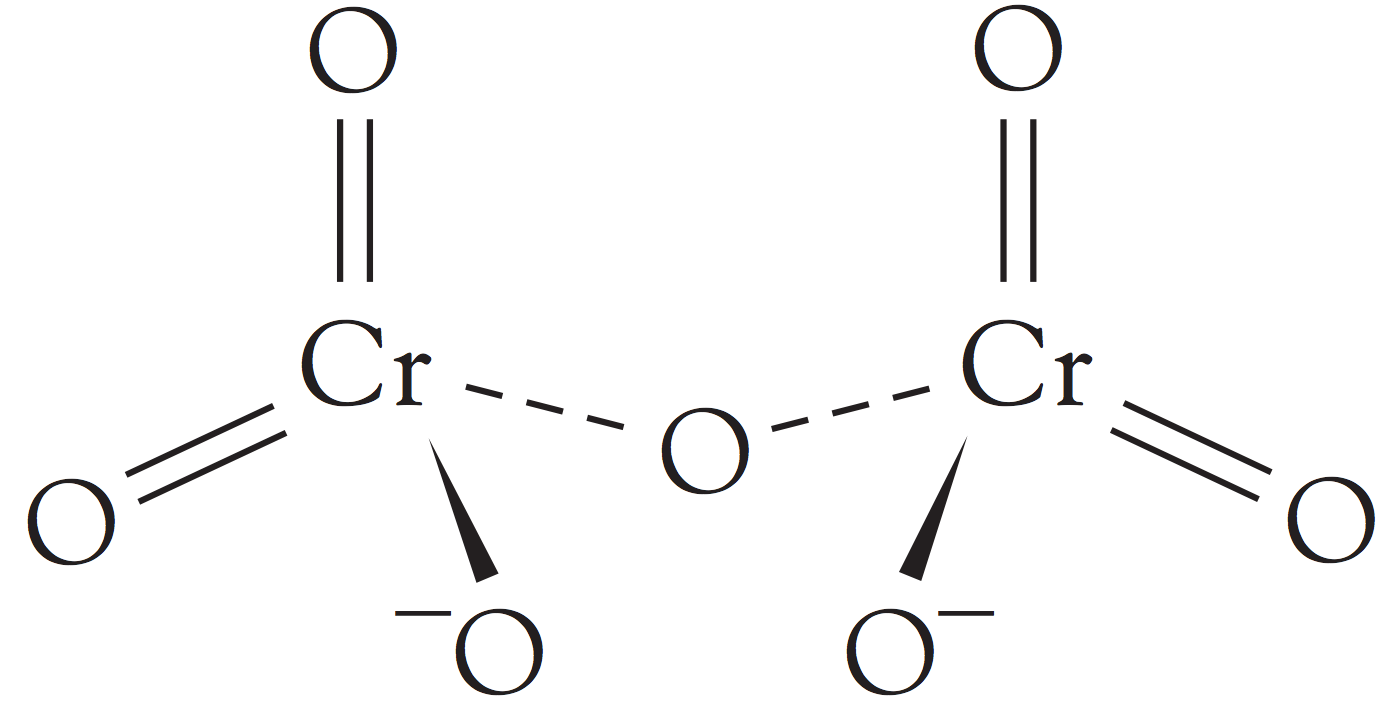
\includegraphics[width=0.9\textwidth]{figures/k20s540dichromat.png}
\end{flashcard}

\begin{flashcard}[Fremstilling]{Angiv hvordan dichromationen fremstilles industrielt}
\ce{4FeCr2O4 + 8Na2CO3 + 7O2 ->[\text{$\Delta$}] 8Na2CrO4 + 2Fe2O3 + 8CO2}\\\vspace*{0.5cm}
\ce{2Na2CrO4 + 2CO2 + H2O <=> Na2Cr2O7 + 2NaHCO3}
\end{flashcard}

\begin{flashcard}[Reaktion]{Angiv hvordan man kan undersøge om der er dichromat i en opløsning}
Dichromationen er orange men reagerer til en blå forbindelse ved tilsætning af hydrogenperoxid og ether.\\\vspace*{0.5cm}
\ce{Cr2O7^{2-} + 4H2O2 + 2H+ -> 2CrO(O2)2(ether) + 5H2O}
\end{flashcard}

\begin{flashcard}[Struktur]{Tegn strukturen af chromylchlorid}
\schemestart
$\chemfig{Cr(=[2]\ce{O})(=[5]\ce{O})(<[:-50]\ce{Cl})(<:[:-12]\ce{Cl})}$
\schemestop
\end{flashcard}

\begin{flashcard}[Fremstilling]{Angiv med en reaktionsligning hvordan man kan fremstille chromylchlorid}
\ce{K2Cr2O7 + 4NaCl + 6H2SO4 -> 2CrO2Cl2 + 2KHSO4 + 4NaHSO4 + 3H2O}
\end{flashcard}

\begin{flashcard}[Reaktion]{Angiv chromylchlorids reaktion i basisk væske}
\ce{CrO2Cl2 + 4OH- -> CrO4^{2-} + 2Cl- + 2H2O}
\end{flashcard}

\begin{flashcard}[Fremstilling]{Hvordan kan man fremstille chrom(VI)oxid?}
\ce{K2Cr2O7 + H2SO4 + H2O -> K2SO4 + "H2CrO4"}\\\vspace*{0.5cm}
\ce{"H2CrO4" -> CrO3 + H2O}
\end{flashcard}

\begin{flashcard}[Anvendelse]{Angiv en karakteristisk anvendelse af chrom(III)oxid}
Chrom(III)oxid er et grønt fast stof som ikke er opløseligt i vand. Derfor anvendes det som pigment i amerikanske dollars.
\end{flashcard}

\begin{flashcard}[Egenskab]{Hvad er den primære mineralkilde til mangan?}
\ce{Mn7SiO12}
\end{flashcard}

\begin{flashcard}[Reaktion]{Kaliumpermangernat kan oxidere saltsyre. Angiv reaktionsligningen}
\ce{2KMnO4 + 16HCl -> 2KCl + 2MnCl2 + 8H2O + 5Cl2}
\end{flashcard}

\begin{flashcard}[Egenskab]{Hvorfor er \ce{Mn^{2+}} næsten farveløs?}
I high spin konfigurationen kan der kun ske elektronovergange ved at vende spinnet af en elektron og parre den med en anden. Sandsynligheden for dette er ekstremt lav da det er en spin forbudt elektronovergang.
\end{flashcard}

\begin{flashcard}[Reaktion]{Mangan(II)hydroxid kan reagere med oxygen. Giv reaktionsligningen}
\ce{4Mn(OH)2(s) + O2 -> 4MnO(OH)(s) + 2H2O}
\end{flashcard}

\begin{flashcard}[Reaktion]{Vis med reaktionsligninger hvorledes man kan undersøge om en opløsning indeholder \ce{Mn^{2+}}}
\ce{2Mn^{2+} + 5 [BiO3]- + 14H+ -> 2MnO4- + 5Bi^{3+} + 7H2O}
\end{flashcard}

\begin{flashcard}[Reaktion]{\ce{Mn2O7} dekomponerer eksplosivt. Giv reaktionsligningen}
\ce{2Mn2O7(l) -> 4MnO2 + 3O2}
\end{flashcard}

\begin{flashcard}[Reaktion]{Ionisk mangan(IV)oxid kan bruges til at fremstille chlorgas. Giv reaktionsligningen}
\ce{MnO2 + 4HCl -> MnCl2 + Cl2 + 2H2O}
\end{flashcard}

\begin{flashcard}[Anvendelse]{Mangan kan anvendes i alkaliske batterier. Opskriv halvcellereaktionerne}
\ce{2MnO2 + 2H2O + 2e- -> 2MnO(OH) + 2OH-}\\
\ce{Zn + 2OH- -> Zn(OH)2(s) + 2e-}
\end{flashcard}

\begin{flashcard}[Fremstilling]{Opskriv reaktionsligningerne til industriel fremstilling af jern ud fra jernmalm i en højovn}
\ce{2C + O2 -> 2CO}\\
\ce{3Fe2O3 + CO -> 2Fe3O4 + CO2}\\
\ce{Fe3O4 + CO -> 3FeO + CO2}\\
\ce{CaCO3 ->[\text{$\Delta$}] CaO + CO2}\\
\ce{FeO + CO -> Fe + CO2}\\
Slagger dannes
\ce{CaO + SiO2 -> CaSiO3}\\
\end{flashcard}

\begin{flashcard}[Fremstilling]{Opskriv reaktionsligningerne til industriel fremstilling af jern ud fra jernmalm af høj kvalitet ved DRI metoden}
\ce{Fe3O4 + CO -> 3FeO + CO2}\\
\ce{Fe3O4 + H2 -> 3FeO + H2O}\\
\ce{FeO + CO -> Fe + CO2}\\
\ce{FeO + H2 -> Fe + H2O}\\
Hydrogen til processen fremstilles via methan reforming\\
\ce{CH4 + CO2 -> 2CO + 2H2}\\
\ce{CH4 + H2O -> CO + 3H2}\\
\end{flashcard}

\begin{flashcard}[Struktur]{Tegn strukturen af \ce{Fe2Cl6}}
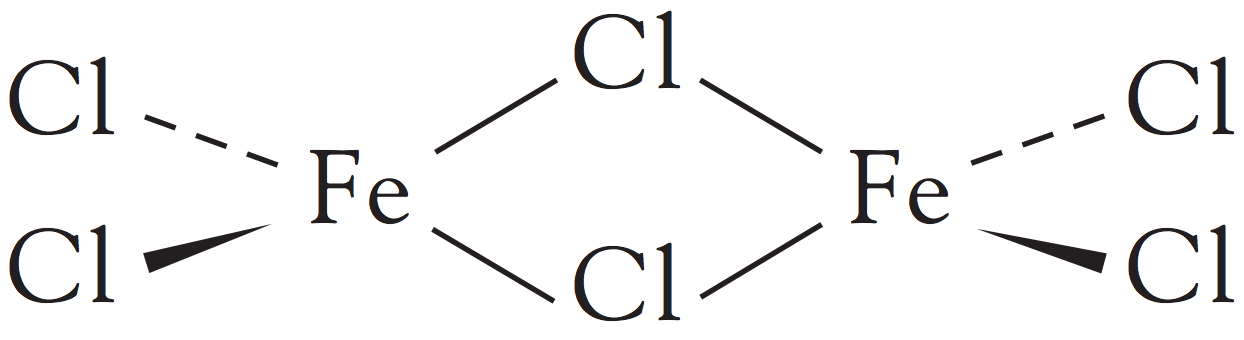
\includegraphics[width=0.9\textwidth]{figures/k20s553fe2cl6.png}
\end{flashcard}

\begin{flashcard}[Reaktion]{Jern kan reagere med chlorgas. Giv reaktionen samt produktets reaktion med vand}
\ce{2Fe + 3Cl2 -> 2FeCl3}\\\vspace*{0.5cm}
\ce{FeCl3 + 3H2O -> Fe(OH)3 + 3HCl(g)}
\end{flashcard}

\begin{flashcard}[Egenskab]{Jern(III) salte regarer ofte surt når de opløses i vand. Hvorfor?}
Ligesom aluminium kan jern koordinere vandmolekyler. På grund af den høje ladningstæthed kan vandmolekylerne binde så stærkt at de kan reagere surt.\\
Eksempelvis:\\
\ce{[Fe(OH2)6]^{3+} + H2O <=> H3O+ + [Fe(OH2)5OH]^{2+}}
\end{flashcard}

\begin{flashcard}[Reaktion]{Jern(III) og jern(II) giver bundfald i basisk væske. Opskriv reaktionsligningerne}
\ce{Fe^{3+} + 3OH- -> FeO(OH) + H2O}\\
Produktet af ovenstående kaldes i daglig tale rust
\ce{Fe^{2+} + 2OH- -> Fe(OH)2}
\end{flashcard}

\begin{flashcard}[Fremstilling]{Angiv reaktionsligningen for industriel fremstilling af jern(II)chlorid}
\ce{Fe + 2HCl(g) -> FeCl2 + H2}
\end{flashcard}

\begin{flashcard}[Reaktion]{Jern(II) og jern(III) kan påvises ved to forskellige lignende metoder der begge giver berlinerblåt. Opskriv reaktionsligningerne}
\ce{3Fe^{2+} + 4[Fe(CN)6]^{3-} -> Fe4[Fe(CN)6]3 + 6CN-}\\\vspace*{0.5cm}
\ce{4Fe^{3+} + 3[Fe(CN)6]^{4-} -> Fe4[Fe(CN)6]3}
\end{flashcard}

\begin{flashcard}[Reaktion]{Opskriv reaktionsligningerne for dannelse af rust}
\ce{2Fe + O2 + 2H2O -> 2Fe(OH)2}\\\vspace*{0.5cm}
\ce{4Fe(OH)2 + O2 -> 4FeO(OH) + 2H2O}
\end{flashcard}

\begin{flashcard}[Reaktion]{Kobolt(II) kan bundfældes med en svag opløsning af stærk base. Herefter går det i opløsning ved kontakt med luft. Giv reaktionsligningerne}
\ce{Co^{2+} + 2OH- -> Co(OH)2}\\\vspace*{0.5cm}
\ce{4Co(OH)2 + O2 -> 4CoO(OH) + 2H2O}
\end{flashcard}

\begin{flashcard}[Fremstilling]{Opskriv reaktionen for oprensning af nikkel ved Mond processen}
\ce{Ni + 4CO <=> Ni(CO)4}\\\vspace*{0.5cm}
Reaktionen er forskudt mod højre ved forholdsvis lave temperaturer
\end{flashcard}

\begin{flashcard}[Egenskab]{Nikkel(II) kan bundfældes med base. Opskriv reaktionen}
\ce{Ni^{2+} + 2OH- -> Ni(OH)2(s)}
\end{flashcard}

\begin{flashcard}[Fremstilling]{Angiv den primære kilde til kobber og hvordan kobberet kan udvindes ved en pyrometallurgisk proces}
\ce{4CuFeS2 + 9O2 -> 2Cu2S + 6SO2 + 2Fe2O3}\\
\ce{Fe2O3 + 3SiO2 -> Fe2(SiO2)3}\\
\ce{2Cu2S + 3O2 -> 2Cu2O + 2SO2}\\
\ce{Cu2S + 2Cu2O -> 6Cu + SO2}
\end{flashcard}

\begin{flashcard}[Fremstilling]{Opskriv reaktionsligningen for udvinding af kobber fra \ce{CuFeS2} ved en hydrometallurgisk proces}
\ce{2CuFeS2 + H2SO4 + 4O2 -> 2CuSO4(aq) + 3S + Fe2O3 + H2O}\\
Kobberet oprenses ved elektrolyse
\end{flashcard}

\begin{flashcard}[Egenskab]{Forklar med udgangspunkt i kobber(II) hvad der forstås ved Jahn-Teller effekten}
$d_{x^2-y^2}$ og $d_{z^2}$ opsplittes i energi fordi der er et ulige antal $d$ elektroner (9) hvorved de to bindinger langs $z$-aksen forlænges.
\end{flashcard}

\begin{flashcard}[Fremstilling]{Hvorledes kan man fremstille kobber(I)chlorid?}
\ce{2Cu + 2H+ -> 2Cu+ + H2}\\
\ce{Cu+ + 2Cl- <=> [CuCl2]-}\\
\ce{[CuCl2]- -> CuCl + Cl-}
\end{flashcard}